
\section{Data illustrations}

\subsection{Simulations}
We have introduced this projected gamma distribution existing on $\mathcal{S}_{\infty}^{p-1}$.  As a
  means of evaluating how well we can recover a distribution under the proposed model, we have
  generated a series of datasets on $\mathcal{S}_{\infty}^{d-1}$, for $d$ ranging between 3 and 20.
  We generated each dataset from a mixture of projected Gammas, with the number of mixture components
  ranging between 3 and 12.  The generation procedure is detailed in Algorithm~\ref{algo:simulated}.
  \begin{algorithm}[htb]
    \For{$n_{\text{mix}}$ in $[3, 6, 9, 12]$}{
      Generate $n_{\text{mix}} \times 20$ shape Parameters $\alpha$\\
      Generate $n_{\text{mix}} \times 20$ Rate Parameters $\beta$\\
      Generate $500$ Mixture Component Identifiers $\delta$\\
      \For{$i$ in $1,\ldots,500$}{
        Generate ${\bf X}_i \sim \prod_{\ell = 1}^d\text{Ga}\left(X_{il}\mid\alpha_{\delta_i,l},\beta_{\delta_i, l}\right)$
        }
      \For{$n_{\text{col}}$ in $[3,6,12,20]$}{
        Project columns 1 to $n_{\text{col}}$ of ${\bf X}$ onto $\mathcal{S}_{\infty}^{n_{\text{col}} - 1}$ and save.
        }
    }
    \caption{Simulated Angular Dataset Generation Routine\label{algo:simulated}}
  \end{algorithm}
  The choice of generation routine for $\alpha = \alpha_0 + \alpha_1$ where
  $\alpha_0 \sim \text{Unif}(\alpha_0\mid 0,4)$, $\alpha_1\sim \text{Gamma}(\alpha_1\mid 1,1)$.
  The choice of generation routine for $\beta$ is $\beta\sim\text{Unif}(\beta\mid 0.25, 2.5)$.
  This choice was made to ensure that $\beta$ does not approach 0 in the generation routine.

\begin{figure}[ht]
  \caption{Simulation Energy Score versus Column Count, by Mixture Component Count.\label{fig:simes}}
  \centering
  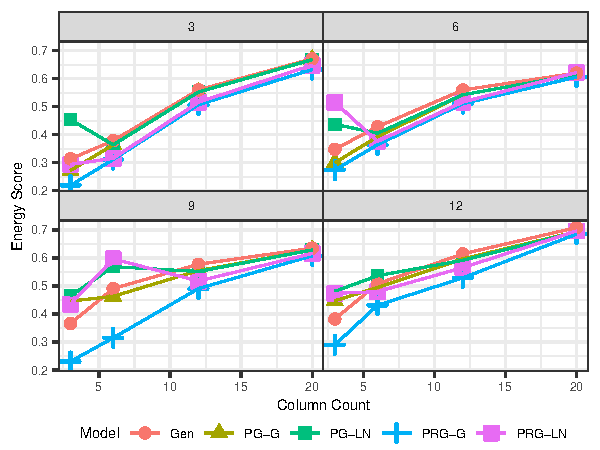
\includegraphics[width=0.8\textwidth]{./images/simulation_es}
\end{figure}

In Figure~\ref{fig:simes}, we fit DP Mixtures of the various models presented and plot the resulting
  energy score against the number of columns, grouped by the number of mixture components used in
  dataset generation.  The \emph{Generative} model refers to a dataset generated
  in the same manner, from the same parameters as was used to create the original dataset.  Against
  this generative dataset, we compare DP Mixtures of projected gamma, projected restricted gamma, and
  projected restricted gamma with a multivariate log-normal prior.  We observe that the projected
  restricted Gamma model dominates in most situations, but the difference between projected restricted
  Gamma and the other gamma-based models tends to shrink as the number of columns increases.
  Alternatively, that difference appears to grow as the number of mixture components increases.

\begin{figure}[ht]
  \caption{Simulation Posterior Predictive Loss versus Column Count, by Mixture Component Count.\label{fig:simppl}}
  \centering
  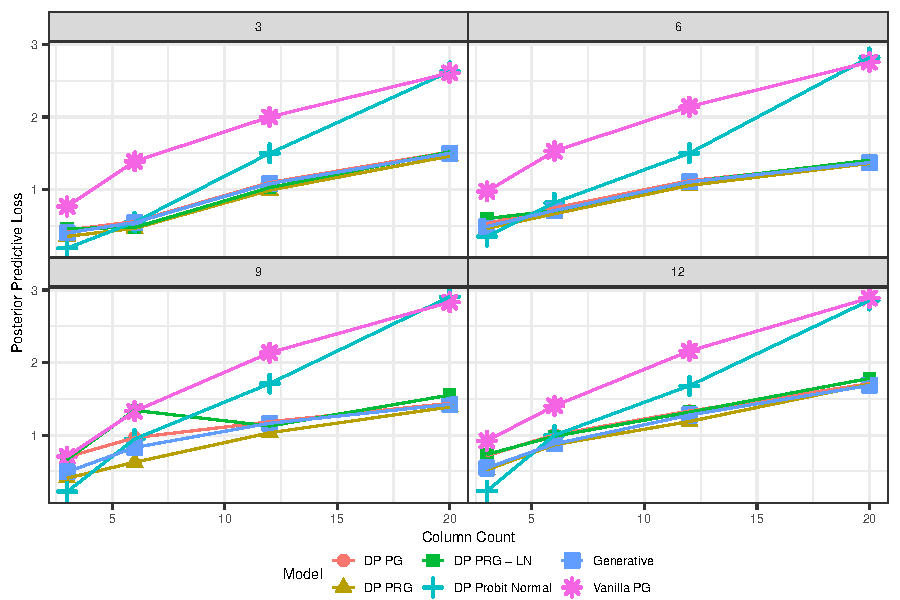
\includegraphics[width=0.8\textwidth]{./images/simulation_ppl}
\end{figure}

The posterior predictive loss criterion in Figure~\ref{fig:simppl} tells a similar story: the base
  model is inadequate for describing a mixture; and the DP mixture of projected restricted gammas
  performs the best of the presented models in most cases.  Interestingly, under both metrics we see
  the probit-normal model has the best performance when the number of columns is low.  That is
  unexpected behavior, as its performance very quickly degrades as the number of columns increases.

We frequently see all of the gamma-based mixture models accomplish a lower energy score than the generative
  distribution.  As \cite{nunez2019} noted, the projected Gamma model is very flexible and can generate
  multimodal distributions from a single mixture component.  When we allow a mixture model, we allow
  the possibility to break those modes into two different mixture components.  This will tend to
  result in a better energy score, as posterior predictive replicates for a given observation in a local
  model will tend to be concentrate in that local mode rather than being spread between multiple
  modes.  As for the dominance of projected restricted Gamma, By specifying $\beta_{\ell} := 1$ for all
  $l$, if there were multi-modal mixture components, we are in effect breaking the mixture components
  into separate modes. As for whether this represents \emph{overfitting}, If we had reason to
  believe that the generative distribution for real data followed this form, then such a case could
  be made.  However, we are using projected Gamma as a parametric stand-in for an unknown distribution.
  In this sense, the argument for overfitting is less clear.

\begin{figure}[ht]
  \caption{Estimated $k$NN-KL Divergence metric on simulated data, averaged between 1 and 10 nearest
    neighbors, against column count, for selected models.  Graphs are facetted according to the
    number of mixture components in the generating distribution.  The \emph{generative} model
    represents another replicate of the underlying distribution, so that should be regarded as
    \emph{truth}.\label{fig:simkld}}
  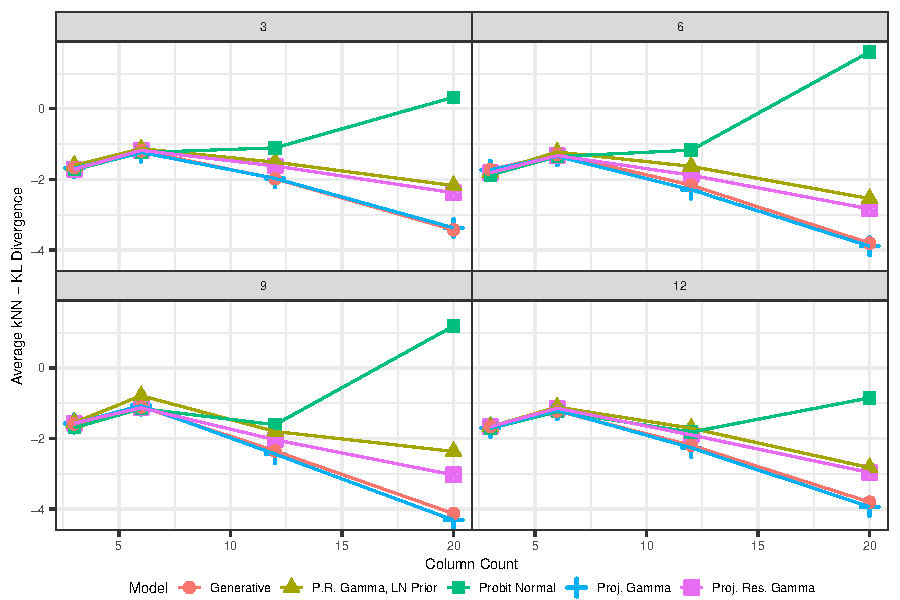
\includegraphics[width = 5.5in, height = 3.75in]{./images/simulation_knn_kld}
\end{figure}

in Figure~\ref{fig:simkld} we see the application of the $k$NN-based K.L. divergence metric detailed
  in Equation~\ref{eqn:knnkld} to the simulated data sets.  For display, this metric has been averaged
  between $1$ and $10$ neighbors.  In general, the K.L. divergence metric is a log-ratio
  of densities, integrated over the entire space.  In this fashion, we should interpret that model
  is \emph{best} that stays closest to 0, as that indicates the two densities are equivalent.  The
  equation also includes a scaling factor for the size of the data sets, as all else being equal, a
  larger data set will decrease the distance between any point and its neighbors.  We can regard the
  \emph{generative} model as another replicate data set from the generating distribution---another
  view of truth.  As its distribution should be almost identical, we would assume that the KL divergence
  metric from this model will come closest to 0.  It does not.  Knowing this to be the case, we should
  instead regard the generative model as truth, and treat as best the model which comes closest to the
  \emph{generative} model.  In this regard, we observe that the projected gamma model comes closest,
  with the projected restricted gamma model following behind.  The probit-normal model quickly diverges
  as the number of dimensions increases.  This is not unexpected, as we saw similar behavior in the
  energy score and posterior predictive loss criteria.

\subsection{Integrated Vapor Transport}
One metric by which we might identify and declare atmospheric rivers is the integrated water vapor
  transport, or \emph{IVT}.  This value represents the total amount of water
  vapor being transported in an atmospheric column---that is, a column of the troposphere above a given
  area of the surface of the Earth. Raw data are measured by dropsondes---measurement devices dropped
  out of aircraft, taking measurements as they fall to the earth.~\citep{ralph2017}  A data vector
  includes an estimate of IVT at grid cell at a period in time; where a grid cell specifies the surface
  of the earth under the atmospheric column.  We have two such datasets, in differing spatial
  resolutions---the lower resolution data splits the coast of california into 8 grid cells, while the
  higher resolution does so into 47 grid cells~\citep{guan2015}.

As IVT tracks water vapor in the atmosphere, extreme values in IVT can lead to
  extreme precipitation events.  Atmospheric rivers are necessary events, in that they carry the
  bulk of precipitation that California recieves, but extreme precipitation events can be extremely
  destructive as well.  Thus, we are interested in the distribution of extreme precipitation events,
  including their depenedence structure.  This tells us about the probability of jointly extreme
  events---where IVT is extreme in two or more grid cells, as well as identifying particular
  configurations of IVT that may be anomalous.  In California, groundwater is a managed resource.
  Extreme precipitation events significantly affect groundwater, so anomalous precipitation events
  can produce anomalous configurations of groundwater, leading to destructive flooding.

We use data from the integrated water vapor transport (\emph{IVT}) model \citep{guan2015}
  of atmospheric rivers as a means of testing these models.  An atmospheric river is a meteorological
  event of local concentration of water vapor in the atmosphere that moves with wind patterns.
  Understanding extremal dependence in atmospheric rivers, for instance, grants hydrological engineers
  a greater understanding of how and where to build ground water capacity to handle precipitation.
  California suffers persistent, extended droughts---if ground water transportation and holding capacity
  (canals, reservoirs) are not built to manage extreme precipitation without adequate understanding of
  the extremal dependence, then we may not install adequate capacity and thus experience flooding.
  Alternatively, if we install too much capacity everywhere, then we are wasting money that could be
  better spent elsewhere.
  
  {\bf We need a one paragraph summary of the stuff in the last three paragraphs. Say what IVT, how it is obtained, why it is important and describe the two datasets you have.}

Fitting our models to this data requires some pre-processing. First, we subset the data to the rainy
  season, which appears from November to March.  The marginal distributions of the
  IVT data appear naturally log-normal, which falls into the domain of attraction of a Gumbel
  distribution.  Given that, we can apply a high threshold, and exceedances over that threshold can
  be modelled as Generalized Pareto.  Our modelling begins with that assessment.  As estimating
  the Pareto parameters is not yet our focus in this analysis, we choose to apply the threshold
  using the empirical CDF.  That is, for a given $t$, let $b_{t,\ell} = \hat{F}_{\ell}^{-1}(1 - t^{-1})$.  For
  this analysis, we set $t = 20$, indicating the marginal $95$ percentile.  The other parameters of the
  generalized Pareto---the scale parameter $\alpha_{\ell}$ and the extremal index $\chi_{\ell}$---are set via
  maximum likelihood.  A fully Bayesian model formulation will allow their varying within a
  distribution, but such a model formulation will not be conducive to fitting by Markov-chain Monte
  Carlo methods.

After the thresholding and maximum likelihood estimation of the parameters of the Pareto, we scale
  the data to the standard multivariate Pareto.  Dividing each standardized observation by its
  $\mathcal{L}_{\infty}$ norm, we project the standardized data onto $\mathcal{S}_{\infty}^{d-1}$.
  Data in sequence represents observations in time, and these are heavily correlated.  As such, we
  choose to \emph{decluster} the observations, such that, by observing a sequence of observations
  $\bm{ z}$ for which $\inorm{z_i} > 1$ for each observation in sequence, we keep only the observation
  with the greatest observed $\mathcal{L}_{\infty}$ norm.  The complete procedure is outlined in
  Algorithm~\ref{algo:processing}.

\begin{algorithm}
  \KwResult{$\bm{ r} : r_i \sim \text{Pareto}(1)$, $\bm{ v} \in \mathcal{S}_{\infty}^{d-1}$}
  \For{$\ell = 1,\ldots,d$}{
    Set $b_{t,\ell} = \hat{F}_{\ell}^{-1}\left(1 - \frac{1}{t}\right)$.\\
    With $\bm{ x}_{\ell} > b_{t,\ell}$, fit $a_{\ell}$, $\chi_{\ell}$ via MLE according to generalized Pareto likelihood.\\
    }
  \For{$i = 1,\ldots,n$}{
    Define $z_{i,\ell} = \left(1 + \xi_{\ell}\frac{x_{i,\ell} - b_{t,\ell}}{a_{\ell}}\right)_{+}^{1/\xi_{\ell}}$\\
    Define $r_i = \pnorm{\bm{ z}_i}{\infty}$, $\bm{ V}_i = \frac{\bm{ z}_i}{\pnorm{\bm{ z}_i}{\infty}}$\\
    }
  Subset $\bm{ r},\bm{ v}$ such that $r_i \geq 1$ for all $r_i\in \bm{r}$.\\
  \If{declustering}{
    \For{$i = 1,\ldots,n$}{
      If $r_i \geq 1$ and $r_{i-1} \geq 1$, drop the lesser (and associated $v_i$) from data set.\\
    }
  }
 \caption{Data preprocessing to isolate and transform data exhibiting extreme behavior.  $r_i$
   represents the radial component, and $\bm{v}_i$ the angular component.  The declustering
   portion is relevant if data is correlated in time.\label{algo:processing}}
\end{algorithm}

We have, at our disposal, two data sets from the IVT model, totalling approximately 30 years of daily
  values omitting leap days.  One records data from 8 grid cells, covering
  generally the coast of California.  The other, with a higher resolution, records data from 47 grid
  cells covering the same area.  For the 8-cell data, after subsetting to the rainy season, we have
  $5587$ observations.  After the data processing steps in Algorithm~\ref{algo:processing}, where we
  omit observations not extreme in any dimension, and decluster temporally correlated data, we are left
  with $511$ observations.  For the 47-cell data, after subsetting to the rainy season, we have $6342$
  observations.  After the same data processing, we are left with
  $532$ observations.  We fit our models to both data sets.

\begin{table}[b]
  \centering
  \caption{Model comparison metrics: Posterior Predictive Loss and Energy Score criteria from fitted
    models against the IVT data.  All presented models are DP mixtures; the \emph{Model} field
    identifies the kernel distribution.  For both criteria, lower is better.
  \label{tab:dev}}
  
\begin{tabular}{ccccc}
\toprule
\multicolumn{1}{c}{ } & \multicolumn{2}{c}{dim = 8} & \multicolumn{2}{c}{dim = 47} \\
\cmidrule(l{3pt}r{3pt}){2-3} \cmidrule(l{3pt}r{3pt}){4-5}
Model & PPL & ES & PPL & ES\\
\midrule
PRG & 0.195 & 0.170 & 1.623 & 0.675\\
PRG-LN & 0.232 & 0.192 & 1.400 & 0.582\\
PG & 0.787 & 0.418 & 5.040 & 1.374\\
\bottomrule
\end{tabular}
\end{table}

In Table~\ref{tab:dev} we see the same model preference towards the projected restricted gamma models
  that we saw in Figures~\ref{fig:simes},\ref{fig:simppl}.  The unrestricted gamma model is penalized much
  more strongly on real data than we saw with our simulation, performing comparably to the probit-normal
  model.  We also see the restricted gamma model with the log-normal prior performing significantly
  better than the restricted gamma model with the gamma prior on the higher dimensional data, a reversal
  of what we saw on the low dimensional data and indeed from what we saw in the simulation study.

That said, there is much we can glean from this table.  The probit-normal model, developed on a
  mapping from $\mathcal{S}_{2}^{d-1}$ to $(-\infty,\infty)^{d-1}$ via probit transformation of
  spherical coordinates was not competitive with the gamma models on real data, similar to what we
  saw in the simulation study. We also established finite mixture models for all presented
  distributions, but after tuning the number of mixture components, their model performance was,
  and could only be \emph{as good} as the DP mixture.  In the interest of parsimony, we only present
  the DP models as representative of mixture distributions.

\begin{figure}[ht]
  \centering
  \caption{KL Divergence Curves calculated through the KNN-KL Metric, evaluated between the
  empirical dataset and posterior predictive datasets of various models.  The top row corresponds
  to the 8-dimensional data, while the bottom row the 47.  All presented models use a DP prior,
  the nominal model being the kernel distribution.\label{fig:knnkl}}
  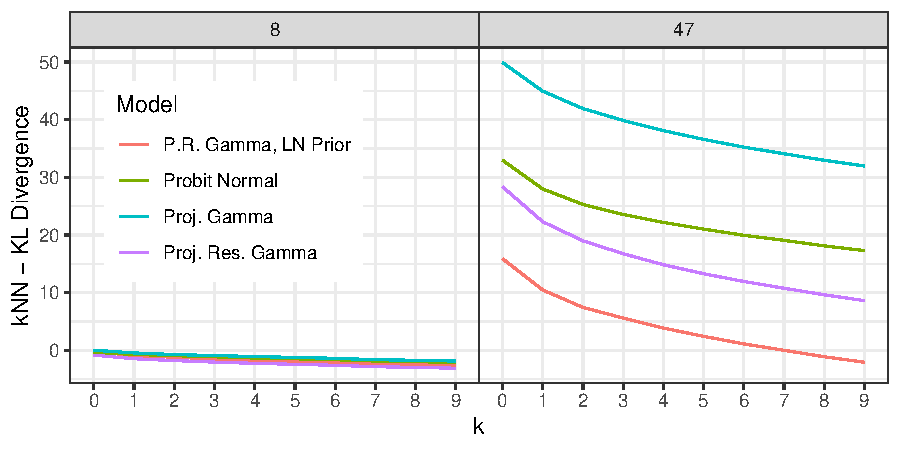
\includegraphics[width = 5.5in, height = 2.75in]{./images/knn_kld}
\end{figure}

Interpreting the KL divergence curves in Figure~\ref{fig:knnkl} is more difficult.  As we saw in
  the simulated case in Figure~\ref{fig:simkld}, the general logic of \emph{best} being that which
  is closest to zero is not necessarily in use here.  We interpret a positive value in the KL
  divergence metric as indicating that, for a given point in the given distribution, we must
  travel \emph{farther} on the target distribution to reach the $k$th neighbor as compared to
  the given distribution.  In this regard, we should regard \emph{large} positive values as
  indicating a particularly poor fit.  By this metric, the projected gamma and probit-normal
  models do not appear to scale well as they performed very poorly on the high dimensional data.
  For the projected restricted gamma model, the log-normal prior appears to scale better than the
  gamma prior.  This is in keeping with what we observed in Table~\ref{tab:dev}, but is a
  different result than what we observed in the simulation study, where we observed that the
  log-normal prior only tended towards the gamma prior, never performing better.

% EOF
